\chapter{DYNAMOS Evaluation}\label{ch:dynamos-evaluation}

This chapter reports the DYNAMOS-specific benchmark used to answer RQ3. The controlled transport benchmark in \Cref{ch:transport-benchmark} isolates communication mechanisms; this chapter evaluates what happens when the selected chunk-aware designs are embedded in the policy-driven DYNAMOS execution path.

\section{Bulk Retrieval Results}\label{sec:dynamos-rq3}

\begin{table}[!htbp]
    \centering
    \scriptsize
    \caption{Average completion latency for DYNAMOS bulk retrieval. All cells completed 20/20 valid repetitions.}
    \label{tab:dynamos-rq3-latency}
    \setlength{\tabcolsep}{3pt}
    \resizebox{\textwidth}{!}{%
    \begin{tabular}{lrrr}
        \toprule
        Implementation & 50k rows & 100k rows & 250k rows \\
        \midrule
        Classic unary & 13.988s & 19.343s & 29.078s \\
        Chunked unary & 6.536s & 6.754s & 11.684s \\
        Intra-job gRPC streaming & 6.346s & 8.255s & 12.319s \\
        RabbitMQ Streams boundary & 5.948s & 7.727s & 14.066s \\
        \bottomrule
    \end{tabular}}
\end{table}

\begin{figure}[!htbp]
    \centering
    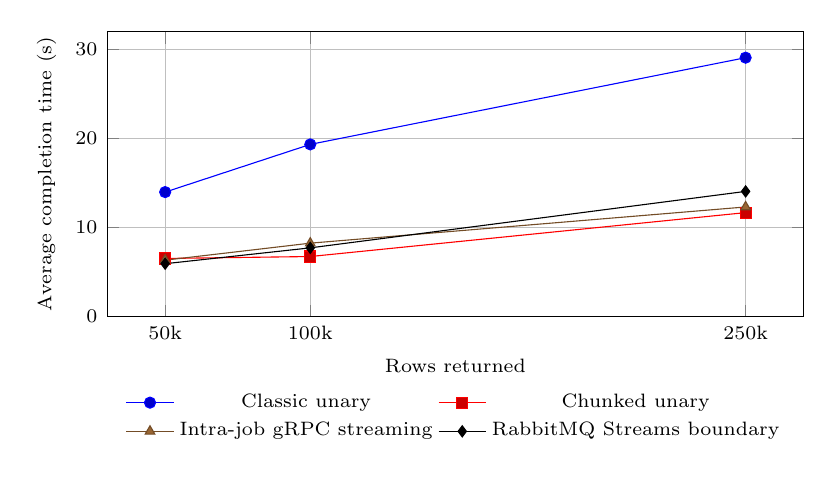
\begin{tikzpicture}
        \begin{axis}[
            width=0.86\textwidth,
            height=5.2cm,
            xlabel={Rows returned},
            ylabel={Average completion time (s)},
            xtick={50000,100000,250000},
            xticklabels={50k,100k,250k},
            scaled x ticks=false,
            ymin=0,
            grid=major,
            legend columns=2,
            legend style={at={(0.5,-0.23)},anchor=north,draw=none},
            tick label style={font=\scriptsize},
            label style={font=\scriptsize},
            legend style={font=\scriptsize}
        ]
            \addplot+[mark=*] coordinates {(50000,13.988) (100000,19.343) (250000,29.078)};
            \addlegendentry{Classic unary}
            \addplot+[mark=square*] coordinates {(50000,6.536) (100000,6.754) (250000,11.684)};
            \addlegendentry{Chunked unary}
            \addplot+[mark=triangle*] coordinates {(50000,6.346) (100000,8.255) (250000,12.319)};
            \addlegendentry{Intra-job gRPC streaming}
            \addplot+[mark=diamond*] coordinates {(50000,5.948) (100000,7.727) (250000,14.066)};
            \addlegendentry{RabbitMQ Streams boundary}
        \end{axis}
    \end{tikzpicture}
    \caption{Average completion time for the local DYNAMOS bulk retrieval benchmark. Chunking is the dominant improvement: all chunk-aware variants scale better than classic unary as the returned row count grows.}
    \label{fig:dynamos-rq3-latency}
\end{figure}

Table~\ref{tab:dynamos-rq3-latency} and Figure~\ref{fig:dynamos-rq3-latency} show that all three chunk-aware variants reduce average completion latency compared with classic unary. At 250k rows, chunked unary is 2.49x faster than classic unary, intra-job gRPC streaming is 2.36x faster, and the RabbitMQ Streams boundary variant is 2.07x faster. The 100k row case is especially favourable to chunked unary, which finishes in 6.754s compared with 19.343s for classic unary. The relatively small increase of the chunked variants between 50k and 100k rows is explained by the fixed control-path cost analysed with Table~\ref{tab:dynamos-rq3-first}: at these sizes much of the measured time is policy handling, orchestration, and job startup rather than transfer.

The average values include the long-tail runs that occur in the local Kubernetes deployment, so they are more conservative than medians. At 250k rows, classic unary ranged from 21.901s to 50.854s. Chunked unary ranged from 7.544s to 23.233s, intra-job gRPC streaming from 7.490s to 23.311s, and RabbitMQ Streams from 9.968s to 26.520s. This spread shows why repeated runs are needed, but the gap between classic unary and the chunked paths is large enough that it does not depend on one unusually fast or slow run.

\section{Additional Scenario Checks}

\begin{table}[!htbp]
    \centering
    \scriptsize
    \caption{Focused DYNAMOS scenario checks beyond the primary single-provider \texttt{dataThroughTtp} benchmark.}
    \label{tab:dynamos-rq3-scenarios}
    \setlength{\tabcolsep}{3pt}
    \resizebox{\textwidth}{!}{%
    \begin{tabular}{llrrrrrr}
        \toprule
        Scenario & Providers & Rows per provider & Total rows & Classic unary & Chunked unary & Intra-job gRPC streaming & RabbitMQ Streams boundary \\
        \midrule
        \texttt{computeToData} & \texttt{UVA,VU} & 50k & 100k & 9.622s & 5.178s & 4.528s & 4.586s \\
        \texttt{computeToData} & \texttt{UVA,VU} & 250k & 500k & 16.620s & 9.182s & 7.989s & 10.289s \\
        \texttt{dataThroughTtp} & \texttt{UVA,VU} & 50k & 100k & 13.750s & 5.196s & 4.474s & 6.492s \\
        \texttt{dataThroughTtp} & \texttt{UVA,VU} & 250k & 500k & 35.396s & 12.032s & 11.165s & 15.618s \\
        \bottomrule
    \end{tabular}}
\end{table}

Table~\ref{tab:dynamos-rq3-scenarios} shows that the chunk-aware paths are not limited to the primary single-provider TTP case. For \texttt{computeToData}, the improvement is smaller because the request avoids part of the TTP aggregation path, but the chunked variants still complete faster than classic unary at both tested sizes. For multi-provider \texttt{dataThroughTtp}, the improvement remains large: at 250k rows per provider, the classic baseline returns 500k total rows in 35.396s, while the chunked variants complete in 11.165s to 15.618s.

These scenario checks are compatibility-oriented rather than an exhaustive benchmark matrix. Their value is that they show the implementation still works when the archetype and provider count change, and that the speedup is strongest when DYNAMOS must move large row sets through the TTP path.

\section{Time to First Result}

\begin{table}[!htbp]
    \centering
    \scriptsize
    \caption{Time-to-first-result and partial result behaviour. Classic unary has no partial results, so first result equals completion.}
    \label{tab:dynamos-rq3-first}
    \setlength{\tabcolsep}{3pt}
    \resizebox{\textwidth}{!}{%
    \begin{tabular}{lrrrrr}
        \toprule
        Implementation & Rows & First result & Done & Post-first & Partial chunks \\
        \midrule
        Classic unary & 50k & 13.988s & 13.988s & 0.000s & 0 \\
        Classic unary & 100k & 19.343s & 19.343s & 0.000s & 0 \\
        Classic unary & 250k & 29.078s & 29.078s & 0.000s & 0 \\
        Chunked unary & 50k & 5.778s & 6.536s & 0.758s & 9 \\
        Chunked unary & 100k & 4.977s & 6.754s & 1.777s & 19 \\
        Chunked unary & 250k & 5.145s & 11.684s & 6.539s & 49 \\
        Intra-job gRPC streaming & 50k & 5.574s & 6.346s & 0.772s & 9 \\
        Intra-job gRPC streaming & 100k & 6.250s & 8.255s & 2.005s & 19 \\
        Intra-job gRPC streaming & 250k & 6.017s & 12.319s & 6.302s & 49 \\
        RabbitMQ Streams boundary & 50k & 5.184s & 5.948s & 0.763s & 9 \\
        RabbitMQ Streams boundary & 100k & 5.416s & 7.727s & 2.311s & 19 \\
        RabbitMQ Streams boundary & 250k & 5.613s & 14.066s & 8.453s & 49 \\
        \bottomrule
    \end{tabular}}
\end{table}

Read as a timeline, the averaged 100k-row chunked-unary request proceeds as follows: the benchmark client submits the HTTP request at $t=0$; policy evaluation, orchestration, generated job creation, pod startup, and initial SQL execution together consume the first ${\sim}5$\,s; the first of 20 chunks reaches the client as a partial \texttt{providerResult} event at $t=5.0$\,s; the remaining 19 chunks drain over the next 1.8\,s; and the final event closes the request at $t=6.8$\,s. The classic unary baseline runs the same control path but stays silent until the single full response at $t=19.3$\,s. The comparison makes the two distinct costs visible: a fixed control-path cost that chunking does not touch, and a transfer-and-buffering cost that it removes almost entirely.

Table~\ref{tab:dynamos-rq3-first} shows the qualitative benefit of chunking. Classic unary cannot expose progress: the first result is the final result. The chunked variants emit partial results substantially earlier. At 250k rows, the first partial result appears after about 5.1s to 6.0s on average, while completion follows after 11.7s to 14.1s. The post-first column estimates how much of the measured time remains after the first visible chunk. It is not a pure network-transfer measurement, because the first chunk still includes policy handling, job creation, and initial SQL execution. It is nevertheless useful because it separates request startup from the observable chunk-drain phase. Read together with Table~\ref{tab:dynamos-rq3-latency}, this decomposition shows that the end-to-end ratios understate the data-path difference: every chunked variant spends roughly 5--6s before the first chunk, which is the shared policy, orchestration, and job-startup cost. End-to-end remains the headline metric since it is what a DYNAMOS client experiences, but the time-to-first-result values show that chunking also changes the interaction pattern: a client can observe progress and begin processing data before the full result has been materialised. This decomposition also matters for diagnosing whether a large request is still making progress.

\section{Resource Usage}

\begin{table}[!htbp]
    \centering
    \scriptsize
    \caption{Peak sampled resource usage during DYNAMOS bulk retrieval. CPU is peak total millicores; memory is peak total MiB across sampled Kubernetes namespaces.}
    \label{tab:dynamos-rq3-resources}
    \setlength{\tabcolsep}{3pt}
    \resizebox{\textwidth}{!}{%
    \begin{tabular}{lrrr}
        \toprule
        Implementation & Rows & Peak CPU & Peak memory \\
        \midrule
        Classic unary & 50k & 958m & 1{,}571 MiB \\
        Classic unary & 100k & 813m & 2{,}046 MiB \\
        Classic unary & 250k & 1{,}198m & 3{,}695 MiB \\
        Chunked unary & 50k & 1{,}059m & 1{,}151 MiB \\
        Chunked unary & 100k & 961m & 1{,}723 MiB \\
        Chunked unary & 250k & 1{,}097m & 1{,}378 MiB \\
        Intra-job gRPC streaming & 50k & 1{,}180m & 1{,}198 MiB \\
        Intra-job gRPC streaming & 100k & 1{,}154m & 1{,}230 MiB \\
        Intra-job gRPC streaming & 250k & 1{,}418m & 1{,}495 MiB \\
        RabbitMQ Streams boundary & 50k & 684m & 1{,}161 MiB \\
        RabbitMQ Streams boundary & 100k & 982m & 1{,}436 MiB \\
        RabbitMQ Streams boundary & 250k & 1{,}687m & 1{,}715 MiB \\
        \bottomrule
    \end{tabular}}
\end{table}

The resource data in Table~\ref{tab:dynamos-rq3-resources} support the main architectural claim. At 250k rows, classic unary reaches 3{,}695 MiB peak memory. Chunked unary stays at 1{,}378 MiB, intra-job gRPC streaming at 1{,}495 MiB, and the RabbitMQ Streams boundary variant at 1{,}715 MiB. Chunking therefore reduces memory pressure across the evaluated row counts.

CPU is more nuanced. Chunked unary uses slightly less peak CPU than classic unary at 250k rows, but intra-job gRPC streaming and the RabbitMQ Streams boundary variant peak higher. This is expected. Chunking replaces one large buffer with more messages, more metadata handling, more serialisation boundaries, and, in the RabbitMQ Streams variant, broker stream handling and reassembly. The defensible claim is therefore that chunking improves latency and memory. CPU remains transport-dependent.

\section{Failure Modes and Robustness}

During the benchmark work, several failure modes had to be controlled before the results could be interpreted reliably. Appendix~\ref{app:dynamos-failure-modes} summarises these cases. The important distinction is that some fixes make the baseline valid, such as correcting the multi-provider merge, while others show the architectural benefit of chunking, such as avoiding single-message size limits and full-result buffering. The RQ3 robustness claim is therefore intentionally bounded: chunking removes size-dependent failure modes, reduces full-result memory pressure, and exposes partial progress, but it does not yet prove recovery from arbitrary pod crashes, broker outages, or mid-stream policy revocation inside DYNAMOS.
